
\usepackage[]{graphicx}\usepackage[]{color}
% maxwidth is the original width if it is less than linewidth
% otherwise use linewidth (to make sure the graphics do not exceed the margin)
\makeatletter
\def\maxwidth{ %
  \ifdim\Gin@nat@width>\linewidth
    \linewidth
  \else
    \Gin@nat@width
  \fi
}
\makeatother

\definecolor{fgcolor}{rgb}{0.345, 0.345, 0.345}
\newcommand{\hlnum}[1]{\textcolor[rgb]{0.686,0.059,0.569}{#1}}%
\newcommand{\hlstr}[1]{\textcolor[rgb]{0.192,0.494,0.8}{#1}}%
\newcommand{\hlcom}[1]{\textcolor[rgb]{0.678,0.584,0.686}{\textit{#1}}}%
\newcommand{\hlopt}[1]{\textcolor[rgb]{0,0,0}{#1}}%
\newcommand{\hlstd}[1]{\textcolor[rgb]{0.345,0.345,0.345}{#1}}%
\newcommand{\hlkwa}[1]{\textcolor[rgb]{0.161,0.373,0.58}{\textbf{#1}}}%
\newcommand{\hlkwb}[1]{\textcolor[rgb]{0.69,0.353,0.396}{#1}}%
\newcommand{\hlkwc}[1]{\textcolor[rgb]{0.333,0.667,0.333}{#1}}%
\newcommand{\hlkwd}[1]{\textcolor[rgb]{0.737,0.353,0.396}{\textbf{#1}}}%
\let\hlipl\hlkwb

\usepackage{framed}
\makeatletter
\newenvironment{kframe}{%
 \def\at@end@of@kframe{}%
 \ifinner\ifhmode%
  \def\at@end@of@kframe{\end{minipage}}%
  \begin{minipage}{\columnwidth}%
 \fi\fi%
 \def\FrameCommand##1{\hskip\@totalleftmargin \hskip-\fboxsep
 \colorbox{shadecolor}{##1}\hskip-\fboxsep
     % There is no \\@totalrightmargin, so:
     \hskip-\linewidth \hskip-\@totalleftmargin \hskip\columnwidth}%
 \MakeFramed {\advance\hsize-\width
   \@totalleftmargin\z@ \linewidth\hsize
   \@setminipage}}%
 {\par\unskip\endMakeFramed%
 \at@end@of@kframe}
\makeatother

\definecolor{shadecolor}{rgb}{.97, .97, .97}
\definecolor{messagecolor}{rgb}{0, 0, 0}
\definecolor{warningcolor}{rgb}{1, 0, 1}
\definecolor{errorcolor}{rgb}{1, 0, 0}
\newenvironment{knitrout}{}{} % an empty environment to be redefined in TeX

\usepackage{alltt}
\newcommand{\SweaveOpts}[1]{}  % do not interfere with LaTeX
\newcommand{\SweaveInput}[1]{} % because they are not real TeX commands
\newcommand{\Sexpr}[1]{}       % will only be parsed by R
\newcommand{\xmark}{\ding{55}}%


\usepackage[english]{babel}
\usepackage[utf8]{inputenc}

\usepackage{dsfont}
\usepackage{verbatim}
\usepackage{amsmath}
\usepackage{amsfonts}
\usepackage{amssymb}
\usepackage{bm}
\usepackage{csquotes}
\usepackage{multirow}
\usepackage{longtable}
\usepackage{booktabs}
\usepackage{enumerate}
\usepackage[absolute,overlay]{textpos}
\usepackage{psfrag}
\usepackage{algorithm}
\usepackage{algpseudocode}
\usepackage{eqnarray}
\usepackage{arydshln}
\usepackage{tabularx}
\usepackage{placeins}
\usepackage{tikz}
\usepackage{setspace}
\usepackage{colortbl}
\usepackage{mathtools}
\usepackage{wrapfig}
\usepackage{bm}
\usepackage{amsmath}
\usepackage{pifont}

\usetikzlibrary{shapes,arrows,automata,positioning,calc,chains,trees, shadows}
\tikzset{
  %Define standard arrow tip
  >=stealth',
  %Define style for boxes
  punkt/.style={
    rectangle,
    rounded corners,
    draw=black, very thick,
    text width=6.5em,
    minimum height=2em,
    text centered},
  % Define arrow style
  pil/.style={
    ->,
    thick,
    shorten <=2pt,
    shorten >=2pt,}
}

\usepackage{subfig}

% Defines macros and environments
\usepackage{../../style/lmu-lecture}


\let\code=\texttt
\let\proglang=\textsf

\setkeys{Gin}{width=0.9\textwidth}

\setbeamertemplate{frametitle}{\expandafter\uppercase\expandafter\insertframetitle}


% basic latex stuff
\newcommand{\pkg}[1]{{\fontseries{b}\selectfont #1}} %fontstyle for R packages
\newcommand{\lz}{\vspace{0.5cm}} %vertical space
\newcommand{\dlz}{\vspace{1cm}} %double vertical space
\newcommand{\oneliner}[1] % Oneliner for important statements
{\begin{block}{}\begin{center}\begin{Large}#1\end{Large}\end{center}\end{block}}





% math spaces
\ifdefined\N
\renewcommand{\N}{\mathds{N}} % N, naturals
\else \newcommand{\N}{\mathds{N}} \fi
\newcommand{\Z}{\mathds{Z}} % Z, integers
\newcommand{\Q}{\mathds{Q}} % Q, rationals
\newcommand{\R}{\mathds{R}} % R, reals
\ifdefined\C
  \renewcommand{\C}{\mathds{C}} % C, complex
\else \newcommand{\C}{\mathds{C}} \fi
\newcommand{\continuous}{\mathcal{C}} % C, space of continuous functions
\newcommand{\M}{\mathcal{M}} % machine numbers
\newcommand{\epsm}{\epsilon_m} % maximum error

% counting / finite sets
\newcommand{\setzo}{\{0, 1\}} % set 0, 1
\newcommand{\setmp}{\{-1, +1\}} % set -1, 1
\newcommand{\unitint}{[0, 1]} % unit interval

% basic math stuff
\newcommand{\xt}{\tilde x} % x tilde
\DeclareMathOperator*{\argmax}{arg\,max} % argmax
\DeclareMathOperator*{\argmin}{arg\,min} % argmin
\newcommand{\argminlim}{\mathop{\mathrm{arg\,min}}\limits} % argmax with limits
\newcommand{\argmaxlim}{\mathop{\mathrm{arg\,max}}\limits} % argmin with limits
\newcommand{\sign}{\operatorname{sign}} % sign, signum
\newcommand{\I}{\mathbb{I}} % I, indicator
\newcommand{\order}{\mathcal{O}} % O, order
\newcommand{\bigO}{\mathcal{O}} % Big-O Landau
\newcommand{\littleo}{{o}} % Little-o Landau
\newcommand{\pd}[2]{\frac{\partial{#1}}{\partial #2}} % partial derivative
\newcommand{\floorlr}[1]{\left\lfloor #1 \right\rfloor} % floor
\newcommand{\ceillr}[1]{\left\lceil #1 \right\rceil} % ceiling
\newcommand{\indep}{\perp \!\!\! \perp} % independence symbol

% sums and products
\newcommand{\sumin}{\sum\limits_{i=1}^n} % summation from i=1 to n
\newcommand{\sumim}{\sum\limits_{i=1}^m} % summation from i=1 to m
\newcommand{\sumjn}{\sum\limits_{j=1}^n} % summation from j=1 to p
\newcommand{\sumjp}{\sum\limits_{j=1}^p} % summation from j=1 to p
\newcommand{\sumik}{\sum\limits_{i=1}^k} % summation from i=1 to k
\newcommand{\sumkg}{\sum\limits_{k=1}^g} % summation from k=1 to g
\newcommand{\sumjg}{\sum\limits_{j=1}^g} % summation from j=1 to g
\newcommand{\meanin}{\frac{1}{n} \sum\limits_{i=1}^n} % mean from i=1 to n
\newcommand{\meanim}{\frac{1}{m} \sum\limits_{i=1}^m} % mean from i=1 to n
\newcommand{\meankg}{\frac{1}{g} \sum\limits_{k=1}^g} % mean from k=1 to g
\newcommand{\prodin}{\prod\limits_{i=1}^n} % product from i=1 to n
\newcommand{\prodkg}{\prod\limits_{k=1}^g} % product from k=1 to g
\newcommand{\prodjp}{\prod\limits_{j=1}^p} % product from j=1 to p

% linear algebra
\newcommand{\one}{\boldsymbol{1}} % 1, unitvector
\newcommand{\zero}{\mathbf{0}} % 0-vector
\newcommand{\id}{\boldsymbol{I}} % I, identity
\newcommand{\diag}{\operatorname{diag}} % diag, diagonal
\newcommand{\trace}{\operatorname{tr}} % tr, trace
\newcommand{\spn}{\operatorname{span}} % span
\newcommand{\scp}[2]{\left\langle #1, #2 \right\rangle} % <.,.>, scalarproduct
\newcommand{\mat}[1]{\begin{pmatrix} #1 \end{pmatrix}} % short pmatrix command
\newcommand{\Amat}{\mathbf{A}} % matrix A
\newcommand{\Deltab}{\mathbf{\Delta}} % error term for vectors

% basic probability + stats
\renewcommand{\P}{\mathds{P}} % P, probability
\newcommand{\E}{\mathds{E}} % E, expectation
\newcommand{\var}{\mathsf{Var}} % Var, variance
\newcommand{\cov}{\mathsf{Cov}} % Cov, covariance
\newcommand{\corr}{\mathsf{Corr}} % Corr, correlation
\newcommand{\normal}{\mathcal{N}} % N of the normal distribution
\newcommand{\iid}{\overset{i.i.d}{\sim}} % dist with i.i.d superscript
\newcommand{\distas}[1]{\overset{#1}{\sim}} % ... is distributed as ...

% machine learning
\newcommand{\Xspace}{\mathcal{X}} % X, input space
\newcommand{\Yspace}{\mathcal{Y}} % Y, output space
\newcommand{\Zspace}{\mathcal{Z}} % Z, space of sampled datapoints
\newcommand{\nset}{\{1, \ldots, n\}} % set from 1 to n
\newcommand{\pset}{\{1, \ldots, p\}} % set from 1 to p
\newcommand{\gset}{\{1, \ldots, g\}} % set from 1 to g
\newcommand{\Pxy}{\mathbb{P}_{xy}} % P_xy
\newcommand{\Exy}{\mathbb{E}_{xy}} % E_xy: Expectation over random variables xy
\newcommand{\xv}{\mathbf{x}} % vector x (bold)
\newcommand{\xtil}{\tilde{\mathbf{x}}} % vector x-tilde (bold)
\newcommand{\yv}{\mathbf{y}} % vector y (bold)
\newcommand{\xy}{(\xv, y)} % observation (x, y)
\newcommand{\xvec}{\left(x_1, \ldots, x_p\right)^\top} % (x1, ..., xp)
\newcommand{\Xmat}{\mathbf{X}} % Design matrix
\newcommand{\allDatasets}{\mathds{D}} % The set of all datasets
\newcommand{\allDatasetsn}{\mathds{D}_n}  % The set of all datasets of size n
\newcommand{\D}{\mathcal{D}} % D, data
\newcommand{\Dn}{\D_n} % D_n, data of size n
\newcommand{\Dtrain}{\mathcal{D}_{\text{train}}} % D_train, training set
\newcommand{\Dtest}{\mathcal{D}_{\text{test}}} % D_test, test set
\newcommand{\xyi}[1][i]{\left(\xv^{(#1)}, y^{(#1)}\right)} % (x^i, y^i), i-th observation
\newcommand{\Dset}{\left( \xyi[1], \ldots, \xyi[n]\right)} % {(x1,y1)), ..., (xn,yn)}, data
\newcommand{\defAllDatasetsn}{(\Xspace \times \Yspace)^n} % Def. of the set of all datasets of size n
\newcommand{\defAllDatasets}{\bigcup_{n \in \N}(\Xspace \times \Yspace)^n} % Def. of the set of all datasets
\newcommand{\xdat}{\left\{ \xv^{(1)}, \ldots, \xv^{(n)}\right\}} % {x1, ..., xn}, input data
\newcommand{\ydat}{\left\{ \yv^{(1)}, \ldots, \yv^{(n)}\right\}} % {y1, ..., yn}, input data
\newcommand{\yvec}{\left(y^{(1)}, \hdots, y^{(n)}\right)^\top} % (y1, ..., yn), vector of outcomes
\newcommand{\greekxi}{\xi} % Greek letter xi
\renewcommand{\xi}[1][i]{\xv^{(#1)}} % x^i, i-th observed value of x
\newcommand{\yi}[1][i]{y^{(#1)}} % y^i, i-th observed value of y
\newcommand{\xivec}{\left(x^{(i)}_1, \ldots, x^{(i)}_p\right)^\top} % (x1^i, ..., xp^i), i-th observation vector
\newcommand{\xj}{\xv_j} % x_j, j-th feature
\newcommand{\xjvec}{\left(x^{(1)}_j, \ldots, x^{(n)}_j\right)^\top} % (x^1_j, ..., x^n_j), j-th feature vector
\newcommand{\phiv}{\mathbf{\phi}} % Basis transformation function phi
\newcommand{\phixi}{\mathbf{\phi}^{(i)}} % Basis transformation of xi: phi^i := phi(xi)

%%%%%% ml - models general
\newcommand{\lamv}{\bm{\lambda}} % lambda vector, hyperconfiguration vector
\newcommand{\Lam}{\bm{\Lambda}}	 % Lambda, space of all hpos
% Inducer / Inducing algorithm
\newcommand{\preimageInducer}{\left(\defAllDatasets\right)\times\Lam} % Set of all datasets times the hyperparameter space
\newcommand{\preimageInducerShort}{\allDatasets\times\Lam} % Set of all datasets times the hyperparameter space
% Inducer / Inducing algorithm
\newcommand{\ind}{\mathcal{I}} % Inducer, inducing algorithm, learning algorithm

% continuous prediction function f
\newcommand{\ftrue}{f_{\text{true}}}  % True underlying function (if a statistical model is assumed)
\newcommand{\ftruex}{\ftrue(\xv)} % True underlying function (if a statistical model is assumed)
\newcommand{\fx}{f(\xv)} % f(x), continuous prediction function
\newcommand{\fdomains}{f: \Xspace \rightarrow \R^g} % f with domain and co-domain
\newcommand{\Hspace}{\mathcal{H}} % hypothesis space where f is from
\newcommand{\fbayes}{f^{\ast}} % Bayes-optimal model
\newcommand{\fxbayes}{f^{\ast}(\xv)} % Bayes-optimal model
\newcommand{\fkx}[1][k]{f_{#1}(\xv)} % f_j(x), discriminant component function
\newcommand{\fh}{\hat{f}} % f hat, estimated prediction function
\newcommand{\fxh}{\fh(\xv)} % fhat(x)
\newcommand{\fxt}{f(\xv ~|~ \thetav)} % f(x | theta)
\newcommand{\fxi}{f\left(\xv^{(i)}\right)} % f(x^(i))
\newcommand{\fxih}{\hat{f}\left(\xv^{(i)}\right)} % f(x^(i))
\newcommand{\fxit}{f\left(\xv^{(i)} ~|~ \thetav\right)} % f(x^(i) | theta)
\newcommand{\fhD}{\fh_{\D}} % fhat_D, estimate of f based on D
\newcommand{\fhDtrain}{\fh_{\Dtrain}} % fhat_Dtrain, estimate of f based on D
\newcommand{\fhDnlam}{\fh_{\Dn, \lamv}} %model learned on Dn with hp lambda
\newcommand{\fhDlam}{\fh_{\D, \lamv}} %model learned on D with hp lambda
\newcommand{\fhDnlams}{\fh_{\Dn, \lamv^\ast}} %model learned on Dn with optimal hp lambda
\newcommand{\fhDlams}{\fh_{\D, \lamv^\ast}} %model learned on D with optimal hp lambda

% discrete prediction function h
\newcommand{\hx}{h(\xv)} % h(x), discrete prediction function
\newcommand{\hh}{\hat{h}} % h hat
\newcommand{\hxh}{\hat{h}(\xv)} % hhat(x)
\newcommand{\hxt}{h(\xv | \thetav)} % h(x | theta)
\newcommand{\hxi}{h\left(\xi\right)} % h(x^(i))
\newcommand{\hxit}{h\left(\xi ~|~ \thetav\right)} % h(x^(i) | theta)
\newcommand{\hbayes}{h^{\ast}} % Bayes-optimal classification model
\newcommand{\hxbayes}{h^{\ast}(\xv)} % Bayes-optimal classification model

% yhat
\newcommand{\yh}{\hat{y}} % yhat for prediction of target
\newcommand{\yih}{\hat{y}^{(i)}} % yhat^(i) for prediction of ith targiet
\newcommand{\resi}{\yi- \yih}

% theta
\newcommand{\thetah}{\hat{\theta}} % theta hat
\newcommand{\thetav}{\bm{\theta}} % theta vector
\newcommand{\thetavh}{\bm{\hat\theta}} % theta vector hat
\newcommand{\thetat}[1][t]{\thetav^{[#1]}} % theta^[t] in optimization
\newcommand{\thetatn}[1][t]{\thetav^{[#1 +1]}} % theta^[t+1] in optimization
\newcommand{\thetahDnlam}{\thetavh_{\Dn, \lamv}} %theta learned on Dn with hp lambda
\newcommand{\thetahDlam}{\thetavh_{\D, \lamv}} %theta learned on D with hp lambda
\newcommand{\mint}{\min_{\thetav \in \Theta}} % min problem theta
\newcommand{\argmint}{\argmin_{\thetav \in \Theta}} % argmin theta

% densities + probabilities
% pdf of x
\newcommand{\pdf}{p} % p
\newcommand{\pdfx}{p(\xv)} % p(x)
\newcommand{\pixt}{\pi(\xv~|~ \thetav)} % pi(x|theta), pdf of x given theta
\newcommand{\pixit}[1][i]{\pi\left(\xi[#1] ~|~ \thetav\right)} % pi(x^i|theta), pdf of x given theta
\newcommand{\pixii}[1][i]{\pi\left(\xi[#1]\right)} % pi(x^i), pdf of i-th x

% pdf of (x, y)
\newcommand{\pdfxy}{p(\xv,y)} % p(x, y)
\newcommand{\pdfxyt}{p(\xv, y ~|~ \thetav)} % p(x, y | theta)
\newcommand{\pdfxyit}{p\left(\xi, \yi ~|~ \thetav\right)} % p(x^(i), y^(i) | theta)

% pdf of x given y
\newcommand{\pdfxyk}[1][k]{p(\xv | y= #1)} % p(x | y = k)
\newcommand{\lpdfxyk}[1][k]{\log p(\xv | y= #1)} % log p(x | y = k)
\newcommand{\pdfxiyk}[1][k]{p\left(\xi | y= #1 \right)} % p(x^i | y = k)

% prior probabilities
\newcommand{\pik}[1][k]{\pi_{#1}} % pi_k, prior
\newcommand{\lpik}[1][k]{\log \pi_{#1}} % log pi_k, log of the prior
\newcommand{\pit}{\pi(\thetav)} % Prior probability of parameter theta

% posterior probabilities
\newcommand{\post}{\P(y = 1 ~|~ \xv)} % P(y = 1 | x), post. prob for y=1
\newcommand{\postk}[1][k]{\P(y = #1 ~|~ \xv)} % P(y = k | y), post. prob for y=k
\newcommand{\pidomains}{\pi: \Xspace \rightarrow \unitint} % pi with domain and co-domain
\newcommand{\pibayes}{\pi^{\ast}} % Bayes-optimal classification model
\newcommand{\pixbayes}{\pi^{\ast}(\xv)} % Bayes-optimal classification model
\newcommand{\pix}{\pi(\xv)} % pi(x), P(y = 1 | x)
\newcommand{\piv}{\bm{\pi}} % pi, bold, as vector
\newcommand{\pikx}[1][k]{\pi_{#1}(\xv)} % pi_k(x), P(y = k | x)
\newcommand{\pikxt}[1][k]{\pi_{#1}(\xv ~|~ \thetav)} % pi_k(x | theta), P(y = k | x, theta)
\newcommand{\pixh}{\hat \pi(\xv)} % pi(x) hat, P(y = 1 | x) hat
\newcommand{\pikxh}[1][k]{\hat \pi_{#1}(\xv)} % pi_k(x) hat, P(y = k | x) hat
\newcommand{\pixih}{\hat \pi(\xi)} % pi(x^(i)) with hat
\newcommand{\pikxih}[1][k]{\hat \pi_{#1}(\xi)} % pi_k(x^(i)) with hat
\newcommand{\pdfygxt}{p(y ~|~\xv, \thetav)} % p(y | x, theta)
\newcommand{\pdfyigxit}{p\left(\yi ~|~\xi, \thetav\right)} % p(y^i |x^i, theta)
\newcommand{\lpdfygxt}{\log \pdfygxt } % log p(y | x, theta)
\newcommand{\lpdfyigxit}{\log \pdfyigxit} % log p(y^i |x^i, theta)

% probababilistic
\newcommand{\bayesrulek}[1][k]{\frac{\P(\xv | y= #1) \P(y= #1)}{\P(\xv)}} % Bayes rule
\newcommand{\muk}{\bm{\mu_k}} % mean vector of class-k Gaussian (discr analysis)

% residual and margin
\newcommand{\eps}{\epsilon} % residual, stochastic
\newcommand{\epsv}{\bm{\epsilon}} % residual, stochastic, as vector
\newcommand{\epsi}{\epsilon^{(i)}} % epsilon^i, residual, stochastic
\newcommand{\epsh}{\hat{\epsilon}} % residual, estimated
\newcommand{\epsvh}{\hat{\epsv}} % residual, estimated, vector
\newcommand{\yf}{y \fx} % y f(x), margin
\newcommand{\yfi}{\yi \fxi} % y^i f(x^i), margin
\newcommand{\Sigmah}{\hat \Sigma} % estimated covariance matrix
\newcommand{\Sigmahj}{\hat \Sigma_j} % estimated covariance matrix for the j-th class

% ml - loss, risk, likelihood
\newcommand{\Lyf}{L\left(y, f\right)} % L(y, f), loss function
\newcommand{\Lypi}{L\left(y, \pi\right)} % L(y, pi), loss function
\newcommand{\Lxy}{L\left(y, \fx\right)} % L(y, f(x)), loss function
\newcommand{\Lxyi}{L\left(\yi, \fxi\right)} % loss of observation
\newcommand{\Lxyt}{L\left(y, \fxt\right)} % loss with f parameterized
\newcommand{\Lxyit}{L\left(\yi, \fxit\right)} % loss of observation with f parameterized
\newcommand{\Lxym}{L\left(\yi, f\left(\bm{\tilde{x}}^{(i)} ~|~ \thetav\right)\right)} % loss of observation with f parameterized
\newcommand{\Lpixy}{L\left(y, \pix\right)} % loss in classification
\newcommand{\Lpiv}{L\left(y, \piv\right)} % loss in classification
\newcommand{\Lpixyi}{L\left(\yi, \pixii\right)} % loss of observation in classification
\newcommand{\Lpixyt}{L\left(y, \pixt\right)} % loss with pi parameterized
\newcommand{\Lpixyit}{L\left(\yi, \pixit\right)} % loss of observation with pi parameterized
\newcommand{\Lhxy}{L\left(y, \hx\right)} % L(y, h(x)), loss function on discrete classes
\newcommand{\Lr}{L\left(r\right)} % L(r), loss defined on residual (reg) / margin (classif)
\newcommand{\lone}{|y - \fx|} % L1 loss
\newcommand{\ltwo}{\left(y - \fx\right)^2} % L2 loss
\newcommand{\lbernoullimp}{\ln(1 + \exp(-y \cdot \fx))} % Bernoulli loss for -1, +1 encoding
\newcommand{\lbernoullizo}{- y \cdot \fx + \log(1 + \exp(\fx))} % Bernoulli loss for 0, 1 encoding
\newcommand{\lcrossent}{- y \log \left(\pix\right) - (1 - y) \log \left(1 - \pix\right)} % cross-entropy loss
\newcommand{\lbrier}{\left(\pix - y \right)^2} % Brier score
\newcommand{\risk}{\mathcal{R}} % R, risk
\newcommand{\riskbayes}{\mathcal{R}^\ast}
\newcommand{\riskf}{\risk(f)} % R(f), risk
\newcommand{\riskdef}{\E_{y|\xv}\left(\Lxy \right)} % risk def (expected loss)
\newcommand{\riskt}{\mathcal{R}(\thetav)} % R(theta), risk
\newcommand{\riske}{\mathcal{R}_{\text{emp}}} % R_emp, empirical risk w/o factor 1 / n
\newcommand{\riskeb}{\bar{\mathcal{R}}_{\text{emp}}} % R_emp, empirical risk w/ factor 1 / n
\newcommand{\riskef}{\riske(f)} % R_emp(f)
\newcommand{\risket}{\mathcal{R}_{\text{emp}}(\thetav)} % R_emp(theta)
\newcommand{\riskr}{\mathcal{R}_{\text{reg}}} % R_reg, regularized risk
\newcommand{\riskrt}{\mathcal{R}_{\text{reg}}(\thetav)} % R_reg(theta)
\newcommand{\riskrf}{\riskr(f)} % R_reg(f)
\newcommand{\riskrth}{\hat{\mathcal{R}}_{\text{reg}}(\thetav)} % hat R_reg(theta)
\newcommand{\risketh}{\hat{\mathcal{R}}_{\text{emp}}(\thetav)} % hat R_emp(theta)
\newcommand{\LL}{\mathcal{L}} % L, likelihood
\newcommand{\LLt}{\mathcal{L}(\thetav)} % L(theta), likelihood
\newcommand{\LLtx}{\mathcal{L}(\thetav | \xv)} % L(theta|x), likelihood
\newcommand{\logl}{\ell} % l, log-likelihood
\newcommand{\loglt}{\logl(\thetav)} % l(theta), log-likelihood
\newcommand{\logltx}{\logl(\thetav | \xv)} % l(theta|x), log-likelihood
\newcommand{\errtrain}{\text{err}_{\text{train}}} % training error
\newcommand{\errtest}{\text{err}_{\text{test}}} % test error
\newcommand{\errexp}{\overline{\text{err}_{\text{test}}}} % avg training error

% lm
\newcommand{\thx}{\thetav^\top \xv} % linear model
\newcommand{\olsest}{(\Xmat^\top \Xmat)^{-1} \Xmat^\top \yv} % OLS estimator in LM


\newcommand{\sens}{\mathbf{A}} % vector x (bold)
\newcommand{\ba}{\mathbf{a}}
\newcommand{\batilde}{\tilde{\mathbf{a}}}
\newcommand{\Px}{\mathbb{P}_{x}} % P_x
\newcommand{\Pxj}{\mathbb{P}_{x_j}} % P_{x_j}
\newcommand{\indep}{\perp \!\!\! \perp} % independence symbol
% ml - ROC
\newcommand{\np}{n_{+}} % no. of positive instances
\newcommand{\nn}{n_{-}} % no. of negative instances
\newcommand{\rn}{\pi_{-}} % proportion negative instances
\newcommand{\rp}{\pi_{+}} % proportion negative instances
% true/false pos/neg:
\newcommand{\tp}{\# \text{TP}} % true pos
\newcommand{\fap}{\# \text{FP}} % false pos (fp taken for partial derivs)
\newcommand{\tn}{\# \text{TN}} % true neg
\newcommand{\fan}{\# \text{FN}} % false neg

\newcommand{\Tspace}{\mathcal{T}}
\newcommand{\tv}{\mathbf{t}}
\newcommand{\tj}{\mathbf{t}_j}
\renewcommand{\l}{L}
\newcommand{\Aspace}{\mathcal{A}}
\newcommand{\Zspace}{\mathcal{Z}}
\newcommand{\norm}[1]{\left|\left|#1\right|\right|_2}


\newcommand{\llin}{\l^{\texttt{lin}}}
\newcommand{\lzeroone}{\l^{0-1}}
\newcommand{\lhinge}{\l^{\texttt{hinge}}}
\newcommand{\lexphinge}{\widetilde{\l^{\texttt{hinge}}}}
\newcommand{\lconv}{\l^{\texttt{conv}}}
\newcommand{\FTL}{\texttt{FTL}}
\newcommand{\FTRL}{\texttt{FTRL}}
\newcommand{\OGD}{{\texttt{OGD}}}
\newcommand{\EWA}{{\texttt{EWA}}} 
\newcommand{\REWA}{{\texttt{REWA}}} 
\newcommand{\EXPthree}{{\texttt{EXP3}}}
\newcommand{\EXPthreep}{{\texttt{EXP3P}}}
\newcommand{\reg}{\psi}
\newcommand{\Algo}{\texttt{Algo}}

\usepackage{multicol}

\newcommand{\titlefigure}{figure/bias-variance-tradeoff}
\newcommand{\learninggoals}{
  \item Get to know the FTL algorithm
  \item See it's flaws and understand the root cause
  \item Get to know the FTRL algorithm as a stable alternative
}

\title{Advanced Machine Learning}
\date{}

\begin{document}

\lecturechapter{Simple Online Learning Algorithms}
\lecture{Advanced Machine Learning}



\sloppy


\begin{frame}
	\frametitle{The online learner}
	%	
	\small
	%	
	\begin{itemize}
		%		
		\item In the following, we will consider a first (online) learner for   online learning problems. Note that a learner can be defined in a formal way.
		%
		\item Indeed, a learner (within the basic online learning protocol), say \Algo, is a function $A: \bigcup_{t=1}^T (\Zspace \times \Aspace)^t \to \Aspace$ that returns the current action based on (the loss $\l$ and) the full history of information so far:
		%		
		$$	a_{t+1}^{\Algo} = A(z_1,a_1^{\Algo},z_2,a_2^{\Algo},\ldots,z_t,a_t^{\Algo};\l).		$$
		%		
		 \item It will be desired that the online learner admits a \emph{cheap update formula}, which is incremental, i.e., only a portion of the previous data is necessary to determine the next action.
		%
		 \item  For instance, there exists a function $u:\Zspace \times \Aspace \to \Aspace$ such that 
		%
		$$	A(z_1,a_1^{\Algo},z_2,a_2^{\Algo},\ldots,z_t,a_t^{\Algo};\l) = u(z_t,a_t^{\Algo}).$$
%		
		\item In the extended online learning scenario, where the environmental data consists of two parts, $z_t=(z_t^{(1)},z_t^{(2)}   ),$ and the {\color{red}first part is revealed before the action in $t$ is performed}, we have that
				%		
				$$	a_{t+1}^{\Algo} =  A(z_1,a_1^{\Algo},z_2,a_2^{\Algo},\ldots,z_t,a_t^{\Algo},{\color{red} z_{t+1}^{(1)}};\l)  		$$
				 
		%
	\end{itemize}
	%	
\end{frame}

\begin{frame} 
	\frametitle{Follow the leader algorithm}
	%	
	\footnotesize
	%
	\begin{itemize}
		%		
		\item A simple algorithm to tackle online learning problems  is the \textbf{Follow the leader} (FTL) algorithm.
		%		
		 \item Suppose that the online learning problem consists of an action space $\Aspace\subset \R^{d_1},$ an environmental space $\Zspace \subset \R^{d_2}$ and some loss function $\l:\Aspace \times \Zspace \to \R$ with $d_1,d_2\in \N.$
		%
		 \item The algorithm takes as its action $a_t^{\FTL} \in \Aspace$ in time step $t \geq 2,$ the element which has the minimal cumulative loss so far over the previous $t-1$ time periods:
		%
		\begin{align*} 
			%		\label{defi_ftl_estimate}
			%	
			a_t^{\FTL} \in \argmin_{a \in \mathcal{A}} \sum_{s=1}^{t-1} \l(a,z_s).
			%	
		\end{align*}
		%
		{\tiny (Technical side note: if there are more than one minimum, then one of them is chosen. Moreover, $a_1^{\FTL}$ is arbitrary. )}
		%		
		 \item \emph{Interpretation:} The  action $a_t^{\FTL}$ is the current ''leader'' of the actions in $\Aspace$ in time step $t$, as it has the smallest cumulative loss (error) so far.
		%		
		{\visible<2>{		\item Note that the action selection rule of FTL is natural and has much in common with the classical batch learning approaches based on empirical risk minimization.
				This results in a first issue regarding the computation time for the action, because the longer we run this algorithm, the slower it becomes (in general) due to the growth of the seen data.}}
	\end{itemize}
	%	
\end{frame}

\begin{frame} 
	\frametitle{FTL: A Helpful Lemma}
	%	
	\small
	%
	 \textbf{Lemma:}
		%	
		Let $a_1^{\FTL}, a_2^{\FTL}, \ldots$ be the sequence of actions used by the FTL algorithm for the environmental data sequence $z_1,z_2,\ldots .$
		%	
		 Then, for all $\tilde a \in \Aspace$ it holds that 
		%	
		\begin{align*}
			%	
			R_T^{\FTL}(\tilde a) 
			%	
			&= \sum\nolimits_{t=1}^T \left(\l(a_t^{\FTL},z_t) - \l(\tilde a,z_t)\right) \\
%			
			& {\color{green} \leq} \sum\nolimits_{t=1}^T \left(\l(a_t^{\FTL},z_t) - \l(a_{t+1}^{\FTL},z_t)\right)\\
%			
			&= {\color{blue} \sum\nolimits_{t=1}^T \l(a_t^{\FTL},z_t) }-  {\color{red}\sum\nolimits_{t=1}^T  \l(a_{t+1}^{\FTL},z_t)}.
			%	
		\end{align*}
		%	
		 In particular,
		%
		\begin{equation*}
			%	
			R_T^{\FTL} \leq \sum\nolimits_{t=1}^T \big(\l(a_t^{\FTL},z_t) - \l(a_{t+1}^{\FTL},z_t))\big).
			%	
		\end{equation*}
		% 
		 \emph{Interpretation}: the regret of the FTL algorithm is {\color{green}bounded} by {\color{blue} the difference of cumulated losses of itself} compared to {\color{red} its one-step lookahead cheater version}.
		%
	%	
\end{frame}

\begin{frame} 
	\frametitle{FTL: A Helpful Lemma}
	%	
	\small
	%
		%		
		\textbf{Proof:}
		%
		%			
		In the following, we denote  $a_1^{\FTL}, a_2^{\FTL}, \ldots$  simply by  $a_1, a_2, \ldots$  	
		
		%
		 First, note that the assertion can be restated as follows
		\begin{equation*}
			%
			\begin{split}
				&\quad \sum\limits_{t=1}^T \left(\l(a_t,z_t) - \l(\tilde a,z_t)\right) \leq \sum\limits_{t=1}^T \left(\l(a_t,z_t) - \l(a_{t+1},z_t)\right) \\
				%&\Leftrightarrow - \sum\limits_{t=1}^T \l(\tilde a,z_t) \leq - \sum\limits_{t=1}^T \l(a_{t+1},z_t) \\
				 &\Leftrightarrow \sum\limits_{t=1}^T \l(a_{t+1},z_t) \leq  \sum\limits_{t=1}^T \l(\tilde a,z_t).
			\end{split} 
			%	
		\end{equation*}
		%
		 Hence, we will verify the inequality $\sum\nolimits_{t=1}^T \l(a_{t+1},z_t) \leq  \sum\nolimits_{t=1}^T \l(\tilde a,z_t),$ which implies the assertion.
		 \lz
		 
		%			 
		 $\leadsto$ This will be done  by induction over $T$.
		%			
	%	
\end{frame}

\begin{frame} 
	\frametitle{FTL: A Helpful Lemma}
	%	
	\small
	%
			\textbf{Initial step: $T=1.$} It holds that
			%
			\begin{equation*}
				%
				\begin{split}
					%
					\sum\limits_{t=1}^T \l(a_{t+1},z_t) 
					%					
					 &= \l(a_2,z_1) 
					 = \l\left(\arg\min\limits_{a \in \Aspace} \l(a,z_1),z_1   \right) \\ 
					%				
					 &= \min\limits_{a \in \Aspace} \l(a,z_1) \leq \l(\tilde a,z_1)  \quad \left(= \sum\nolimits_{t=1}^T \l(\tilde a,z_t) \right)
					%				\quad \forall \tilde a \in \Aspace.
					%
				\end{split} 
				%
			\end{equation*} 
			%
			for all $\tilde a  \in \Aspace$. 
			%	
			{\visible<2>{ \textbf{Induction Step: $T -1 \rightarrow T.$}
			%
			Assume  that for any $\tilde a  \in \Aspace$ it holds that 
			%
			\begin{equation*}
				%
				\sum\nolimits_{t=1}^{T-1} \l(a_{t+1},z_t) \leq  \sum\nolimits_{t=1}^{T-1} \l(\tilde a,z_t).
				%
			\end{equation*}
			%
			 Then, the following holds as well (adding $\l(a_{T+1},z_T)$ on both sides)
			%
			\begin{equation*}
				%
				\begin{split}
					%	
					%		&\quad \sum\limits_{t=1}^{T-1} \l(a_{t+1},z_t) \leq  \sum\limits_{t=1}^{T-1} \l(\tilde a,z_t) \\
					%		&\Leftrightarrow \l(a_{t+1},z_t) + \sum\limits_{t=1}^{T-1} \l(a_{t+1},z_t) \leq  \l(a_{t+1},z_t) + \sum\limits_{t=1}^{T-1} \l(\tilde a,z_t)\\
					%		&\Leftrightarrow 
					\sum\nolimits_{t=1}^{T} \l(a_{t+1},z_t) \leq \l(a_{T+1},z_T) + \sum\nolimits_{t=1}^{T-1} \l(\tilde a,z_t), \quad \forall \tilde a  \in \Aspace.
					%		
				\end{split}
				%
			\end{equation*}}}
			
%		\end{itemize}
%	\end{itemize}
	%	
\end{frame}

\begin{frame} 
	\frametitle{FTL: A Helpful Lemma}
	%	
	\small
	%
			\begin{equation*}
				%
				\begin{split}
					%	
					\mbox{\textbf{Reminder:} \qquad }\sum\nolimits_{t=1}^{T} \l(a_{t+1},z_t) \leq \l(a_{T+1},z_T) + \sum\nolimits_{t=1}^{T-1} \l(\tilde a,z_t).
					%		
				\end{split}
				%
			\end{equation*} 
			
			{\visible<2>{  Using the latter inequality with  $\tilde a = a_{T+1}$ yields
			%		
			\begin{align*}\allowdisplaybreaks
				%\begin{split}
				%
				%	&\quad \sum\limits_{t=1}^{T} \l(a_{t+1},z_t) \leq \l(a_{T+1},z_T) + \sum\limits_{t=1}^{T-1} \l(\tilde a,z_t) \\
				%%	
				%	&\Leftrightarrow \sum\limits_{t=1}^{T} \l(a_{t+1},z_t) \leq \l(a_{T+1},z_T) + \sum\limits_{t=1}^{T-1} \l(a_{T+1},z_t) \\
				%%	
				%	&\Leftrightarrow 
				\sum\limits_{t=1}^{T} \l(a_{t+1},z_t) 
				%				
				&\leq \sum\limits_{t=1}^{T} \l(a_{T+1},z_t) 
				 = \sum\limits_{t=1}^{T} \l\Big(\arg\min\limits_{a \in \mathcal{A}} \sum\limits_{t=1}^T \l(a,z_t),z_t\Big) \\
				%	
				%	&\Leftrightarrow \sum\limits_{t=1}^{T} \l(a_{t+1},z_t)
				 &= \min\limits_{a \in \mathcal{A}}  \sum\limits_{t=1}^{T}\l(a,z_t) 
				%	 
				 \leq \sum\limits_{t=1}^{T}\l(\tilde a,z_t)
				%\end{split}
			\end{align*} 
			%
			for all $\tilde a \in \Aspace.$
			%	This completes the proof.
			\qed }}
			%			
			%			
			%			
			%			
			%			
		
	%	
\end{frame}




\begin{frame} 
	\frametitle{FTL for OQO problems}
	%	
	\footnotesize
%
	\begin{itemize}
%		
		\item One popular instantiation of the online learning problem is the problem of \emph{online quadratic optimization} (OQO).
		%		
		\item In its most general form, the loss function is thereby defined as 
		%	
		\begin{align*}
			%		 \label{defi_loss_quadratic_optim}
			%		
			\l(a_t,z_t) =  \frac12 \norm{a_t-z_t}^2,
			%		
		\end{align*}
%	
		where $\Aspace$ and $\Zspace$ have the same dimensionality.
%		
		%		
	 	\item  {\visible<2->{ \textbf{Proposition:}
		%	
		Using FTL on any online quadratic optimization problem with $\Aspace = \mathbb{R}^d$ and $V = \sup\limits_{z \in \Zspace} \norm{z}$, leads to a regret of  
		%	 
		\begin{equation*}
			%	
			R_T^{\FTL}  \leq 4V^2 \, (\log(T) + 1 ).
			%		
		\end{equation*} }}
		%
	 	\item {\visible<3>{ This result is satisfactory for three reasons:
%		
		\begin{itemize}\footnotesize
			%			
			\item  The regret is definitely sublinear, that is,	$R_T^{\FTL}  = o(T).$
			%			
			\item  We just have a mild constraint on the online quadratic optimization problem, namely that $
			\norm{z} \leq V$ holds for any possible environmental data instance $z\in \Zspace.$
			%			
			\item The action $a_t^{\FTL}$ is simply the empirical average of the environmental data seen so far: $a_t^{\FTL} = \frac{1}{t-1}\sum_{s=1}^{t-1} z_s.$
			%		
		\end{itemize}   }}
		%	
		
	\end{itemize}
	%	
\end{frame}


%\begin{frame} 
%	\frametitle{FTL for OQO problems: Theoretical guarantees}
%	%	
%	\small
%	\begin{itemize}		
%		
%		\item \textbf{Proof:}
%		%	
%		\begin{itemize}
%			%				
%			\item In the following, we denote  $a_1^{\FTL}, a_2^{\FTL}, \ldots$  simply by  $a_1, a_2, \ldots$  	
%			%			
%			 \item  Using the {\color{blue} lemma} for the comparison of FTL with its one-step lookahead cheater version, we just have to show that
%			%
%			\begin{align} \label{ineq_help_FTL_quadr}
%				%	
%				\sum\limits_{t=1}^T \left(\l(a_t,z_t) - \l(a_{t+1},z_t)  \right) \leq 4L^2 \cdot \left(\log(T) + 1 \right),
%				%	
%			\end{align}
%			%						
%			since $R_T^{\FTL} \stackrel{{\color{blue} \mbox{Lemma}}}{\leq} \sum\nolimits_{t=1}^T \left(\l(a_t,z_t) - \l(a_{t+1},z_t)  \right).$ 
%			%				
%			 \item So, we will prove (\ref{ineq_help_FTL_quadr}).
%			%				
%			For this purpose, we compute the explicit form of the actions of FTL for this type of online learning problem.
%			%				
%		\end{itemize}
%		%		
%	\end{itemize}
%\end{frame}
%
%
%\begin{frame} 
%	\frametitle{FTL for OQO problems: Theoretical guarantees}
%	%	
%	\small
%	\begin{itemize}	
%		%	
%		\item[]
%		\begin{itemize}	
%			%				
%			\item Claim: It holds that $a_t = \frac{1}{t - 1} \cdot \sum\nolimits_{s = 1}^{t-1} z_s,$ if $\l(a,z)=\frac12\norm{a-z}^2 .$ 
%			%				
%			\begin{itemize}
%				%				
%				 \item	Recall that $$a_t^{\FTL} = \argmin{a \in \mathcal{A}} \sum_{s=1}^{t-1} \l(a,z_s)  = \argmin{a \in \mathcal{A}} \sum_{s=1}^{t-1} \frac12 \norm{a - z_s}^2. $$
%				%						
%				 \item So, we have to find the minimizer of the function $$f(a):= \sum_{s=1}^{t-1} \frac12 \norm{a - z_s}^2  =   \sum_{s=1}^{t-1} \frac12 (a - z_s)^\top (a-z_s).$$
%				%						
%				 \item Compute  $\nabla f(a) = \sum_{s=1}^{t-1}  a  - z_s =  (t-1) a  - \sum_{s=1}^{t-1} z_s,$ which we set to zero and solve with respect to $a$ to obtain the claim.\\
%				%
%				{\tiny (The Hessian of $f$ is semi-positive definite, so that this leads indeed to a minimizer.)}
%				%	
%				%				
%			\end{itemize} 
%			%				
%		\end{itemize}
%		%		
%	\end{itemize}
%\end{frame}
%
%
%\begin{frame} 
%	\frametitle{FTL for OQO problems: Theoretical guarantees}
%	%	
%	\small
%	\begin{itemize}	
%		%	
%		\item[]
%		\begin{itemize}	 
%			%
%			\item Hence, $a_t$ is the empirical average of $z_1, \ldots, z_{t-1}$ and we can provide the following incremental update formula for its computation
%			%
%			\begin{equation*}
%				%
%				\begin{split}
%					%	
%					a_{t+1} &= \frac{1}{t} \cdot \sum\limits_{s = 1}^{t} z_s
%					%	
%					 = \frac{1}{t}(z_t + (t-1) a_t) 
%					%	
%					 =  \frac{1}{t} z_t + \left(1 - \frac{1}{t} \right)  a_t.
%					%	
%				\end{split}
%				%
%			\end{equation*} 
%			%
%			%
%			 \item From the last display we derive that
%			%
%			\begin{equation*}
%				%	
%				\begin{split}
%					% 
%					a_{t+1} - z_t = \left(1 - \frac{1}{t} \right) \cdot a_t + \frac{1}{t} z_t - z_t = \left(1 - \frac{1}{t} \right) \cdot (a_t - z_t).
%					%
%				\end{split}
%				%	
%			\end{equation*}
%			%			
%			 \item Claim:
%			%
%			\begin{align*} 
%				%				\label{help_ineq_FTL_analysis}
%				%	
%				\l(a_t,z_t) - \l(a_{t+1},z_t) \leq \frac{1}{t} \cdot \norm{a_t - z_t}^2. \tag{2}
%				%	
%			\end{align*}
%			%	
%		\end{itemize}
%		%
%	\end{itemize}
%\end{frame}
%
%
%\begin{frame} 
%	\frametitle{FTL for OQO problems: Theoretical guarantees}
%	%	
%	\small
%	\begin{itemize}	
%		%	
%		\item[]
%		\begin{itemize}	 
%			%
%			Indeed, this can be seen as follows
%			%
%			{\footnotesize
%				\begin{align*}
%					%
%					\l(a_t,z_t) - \l(a_{t+1},z_t) 
%					%
%					&= \frac{1}{2}\norm{a_t - z_t}^2 - \frac{1}{2}\norm{a_{t+1} - z_{t}}^2 \\
%					%
%					 &= \frac{1}{2} \left( \norm{a_t - z_t}^2 - \norm{a_{t+1} - z_{t}}^2 \right) \\
%					%
%					%				\Big[\mbox{Using \ }a_{t+1} - z_t  = \left(1 - \frac{1}{t} \right) \cdot (a_t - z_t) \Big] \quad  
%					 &= \frac{1}{2} \left( \norm{a_t - z_t}^2  - \norm{\left(1 - \frac{1}{t} \right) \cdot (a_t - z_t)}^2 \right) \\
%					%
%					 &= \frac{1}{2} \left( \norm{a_t - z_t}^2  - \left(1 - \frac{1}{t} \right)^2 \cdot \norm{a_t - z_t}^2 \right) \\
%					%
%					 &= \frac{1}{2} \left(1 - \left(1 - \frac{1}{t} \right)^2 \right) \cdot \norm{a_t - z_t}^2 \\
%					%
%					 &= \left(\frac{1}{t} - \frac{1}{2t^2}\right) \cdot \norm{a_t - z_t}^2 \\
%					%
%					 &\leq \frac{1}{t} \cdot \norm{a_t - z_t}^2.
%					%
%				\end{align*}	
%			}
%			%
%		\end{itemize}
%	\end{itemize}
%\end{frame}
%
%
%\begin{frame} 
%	\frametitle{FTL for OQO problems: Theoretical guarantees}
%	%	
%	\small
%	\begin{itemize}	
%		%	
%		\item[]
%		\begin{itemize}	
%			\footnotesize
%			
%			\item Since by assumption $L = \sup\limits_{z \in \Zspace} \norm{z}$ and $a_t$ is the empirical average of $z_1, \ldots, z_{t-1}$, we have that $\norm{a_t} \leq L.$
%			%
%			 \item Now the triangle inequality states that for any two vectors $x, y \in \mathbb{R}^d$ it holds that 
%			%
%			\begin{equation*}
%				\norm{x + y} \leq \norm{x} + \norm{y},
%			\end{equation*} 
%			%
%			 so that
%			%
%			\begin{equation*} 
%				%				\label{help_ineq_FTL_analysis_sec}
%				%
%				\norm{a_t - z_t} \leq \norm{a_t} + \norm{z_t} \leq 2L.
%				%
%				\tag{3}
%			\end{equation*}
%			%				 
%			 \begin{align}
%				%				 \label{help_ineq_FTL_analysis}
%				%	
%				\mbox{\textbf{Reminder:} \quad }\l(a_t,z_t) - \l(a_{t+1},z_t) \leq \frac{1}{t} \cdot \norm{a_t - z_t}^2 \tag{2}.
%				%	
%			\end{align}	 
%			%
%			 \item Summing over all $t$ in (2) and using (3) we arrive at
%			%
%			\begin{equation*}
%				%
%				\begin{split}
%					%
%					\sum\limits_{t=1}^T \left(\l(a_t,z_t) - \l(a_{t+1},z_t)  \right) 
%					%					
%					 &\leq \sum\limits_{t=1}^T \left(\frac{1}{t} \cdot \norm{a_t - z_t}^2 \right) 
%					%
%					 \leq  \sum\limits_{t=1}^T \frac{1}{t} \cdot (2L)^2 
%					%					
%					 = 4L^2 \cdot \sum\limits_{t=1}^T \frac{1}{t}.
%					%
%					%				\leq 4L^2 \cdot \left(\log(T) + 1 \right),
%					%
%				\end{split}
%				%
%				%
%			\end{equation*}
%			
%		\end{itemize}
%	\end{itemize}
%\end{frame}
%
%
%\begin{frame} 
%	\frametitle{FTL for OQO problems: Theoretical guarantees}
%	%	
%	\small
%	\begin{itemize}	
%		%	
%		\item[]
%		\begin{itemize}	
%			\item[]
%			%				
%			\begin{equation*}
%				%
%				\begin{split}
%					%
%					\mbox{\textbf{Reminder:} \quad } \sum\limits_{t=1}^T \left(\l(a_t,z_t) - \l(a_{t+1},z_t)  \right) 
%					%
%					\leq  4L^2 \cdot \sum\limits_{t=1}^T \frac{1}{t} 
%					%
%					%				\leq 4L^2 \cdot \left(\log(T) + 1 \right),
%					%
%				\end{split}
%				%
%				%
%			\end{equation*}
%			%			
%			%
%			 \item Now, it holds that   $\sum\limits_{t=1}^T \frac{1}{t} \leq \log(T) + 1,$ so that we obtain
%			%				
%			 \begin{equation*}
%				%
%				\begin{split}
%					%
%					\sum\limits_{t=1}^T \left(\l(a_t,z_t) - \l(a_{t+1},z_t)  \right) 
%					%					
%					 &\leq 4L^2 \cdot \sum\limits_{t=1}^T \frac{1}{t} 
%					%
%					  \leq  4L^2 \cdot \left(\log(T) + 1 \right),
%					%
%				\end{split}
%				%
%				%
%			\end{equation*}
%			%
%			which is what we wanted to prove. \qed
%			%
%		\end{itemize}
%		%		
%	\end{itemize}
%	%	
%\end{frame}

\begin{vbframe} \frametitle{FTL for online linear optimization}
	%	 
	\small
	\begin{itemize}
		%	 	
		\item Another popular instantiation of the online learning problem is the online linear optimization problem, which is characterized by a linear loss function $\l(a,z)=a^\top z.$ 
		%	 	
		 \item  Let $\Aspace=[-1,1]$ and  suppose that 
		%	
		$  z_t = \begin{cases}
			-\frac12, & \mbox{$t=1,$} \\
			%			
			1, & \mbox{$t$ is even,}\\
			%			
			-1, & \mbox{$t$ is odd.}
		\end{cases} $
		%	
		 \item No matter how we choose the first action $a_1^{\FTL},$ it will hold that FTL has a cumulative loss greater than (or equal) $T-3/2,$ while the best action in hindsight has a cumulative loss of $-1/2.$ 
%		 
		\item Thus, FTL's cumulative regret is at least $T-1,$ which is linearly growing in $T.$
%		 
		\scriptsize
		\item Indeed, note that 
%		
		\begin{align*}
%			
			a_{t+1}^{\FTL} = \argmin_{a \in \Aspace} \sum_{s=1}^t \l(a,z_s) &= \argmin_{a \in [-1,1]} a \sum_{s=1}^t  z_s \\
			%		
			&= \begin{cases}
				%			
				-1, & \mbox{if }\sum_{s=1}^t  z_s>0,\\
				1, & \mbox{if }\sum_{s=1}^t  z_s<0,\\
				\mbox{arbitrary}, & \mbox{if }\sum_{s=1}^t  z_s=0.\\
				%			
			\end{cases} 
%			
		\end{align*}
		 
		\begin{centering}
			 \begin{tabular}{c|c|c|c|c|c} 
				$t$ & $a_t^{\FTL}$ & $z_t$ & $\l(a_t^{\FTL},z_t)$  &  $\sum_{s=1}^t \l(a_s^{\FTL},z_s)$ & $\sum_{s=1}^t z_s $ \\
				\hline
				1 & 1 & $-1/2$ & $-1/2$ & $-1/2$ & $-1/2$  \\
				\hline
				2 & 1 & 1 & 1 & 1 $- 1/2$ & 1/2 \\
				\hline
				3 & $-1$ & $-1$ & 1 & 2 $- 1/2$ & $-1/2$ \\
				\hline
				\vdots & \vdots & \vdots & \vdots & \vdots & \vdots \\
				\hline 
				& & & & &\\
				$T$ & $(-1)^T$ & $(-1)^T$ & 1 & $T-1-1/2$ & $(-1/2)^{T}$ \\
			\end{tabular}
		\end{centering}
%		 
		\item The best action has cumulative loss 		
%		
		\begin{align*}
			%			
			\inf_{a \in \Aspace} \sum\nolimits_{s=1}^T \l(a,z_s) &= \inf_{a \in [-1,1]} a \underbrace{\sum\nolimits_{s=1}^T  z_s}_{=(-1/2)^{T}} = -1/2.
			%			
		\end{align*}
		%	 	
		\small
%		
		 \item Thus, we see: FTL can fail for {\color{red} online linear optimization problems}, although it is well suited for {\color{blue}  online quadratic optimization problems}!
		%		
		 \item The reason is that the action selection of FTL is not stable enough (caused by the loss function), which is fine for {\color{blue} the latter problem}, but problematic for {\color{red} the former}.
		%
		\item One has to note that the online linear optimization problem example above, where FTL fails, is in fact an adversarial learning setting: The environmental data is generated in such a way that the FTL learner is fooled in each time step.
%		
	\end{itemize}
	%	
\end{vbframe}



\begin{frame} 
	\frametitle{Follow the regularized leader}
	% 	
	\small
	\begin{itemize}
		% 		
		\item To overcome the shortcomings of the FTL algorithm, one can incorporate a regularization function $\reg: \Aspace \to \R_+$ into the action choice of FTL, which leads to more stability.
		% 		
		 \item  
		To be more precise, let for $t\geq 1$
		%
		{\footnotesize 		\begin{align*} 
				%		\label{defi_forel_estimate}
				%	
				a_t^{\FTRL} \in \argmin_{a \in \mathcal{A}} \left( \reg(a) + \sum\nolimits_{s=1}^{t-1} \l(a,z_s) \right),
				%	
			\end{align*}
			{\tiny (Technical side note: if there are more than one minimum, then one of them is chosen.)\\}	
		}
		%
		\noindent then the algorithm choosing $a_t^{\FTRL}$ in time step $t$ is called the \textbf{Follow the regularized leader} (FTRL) algorithm.
		% 		
		  \item {\visible<2->{  \emph{Interpretation:} The algorithm predicts $a_t$ as the element in $\Aspace,$ which minimizes the regularization function plus the cumulative loss so far over the previous $t-1$ time periods.}}
		%		
		  \item {\visible<3>{  Obviously, the behavior of the FTRL algorithm is depending heavily on the choice of the regularization function $\reg.$ 
%		  
		  If $\reg \equiv 0,$ then FTRL equals FTL.}}
	\end{itemize}
	% 	
\end{frame}

\begin{frame} 	
	\frametitle{Regularization in online learning vs.\ batch learning}
	\small
	\begin{itemize}
		%	
		\item Note that in the batch learning scenario, i.e., where training phase and testing phase are decoupled and training data is available before the testing phase, the learner seeks to optimize an objective function which is the sum of the training loss and a regularization function:
		%
		\begin{align*}
			% 		 \label{def:form_of_ml_problems}
			%	
			\min_{\thetab\in \R^p} \, \sum_{i=1}^n L(\yi,\thetab) + \lambda \, \psi(\thetab),	
			%	
		\end{align*}	
		% 		
		where $\lambda\geq 0$ is some regularization parameter.
		%	
		{\visible<2->{  \item Here, the regularization function is part of the whole objective function, which the learner seeks to minimize. }}
		%	
		 \item {\visible<3>{  However, in the online learning scenario the regularization function does (usually) not appear in the regret the learner seeks to minimize, but the regularization function is only part of the action/decision rule at each time step.}}
		% 		
	\end{itemize}
	% 	
\end{frame}


\begin{frame} 
	\frametitle{Regret analysis of FTRL: A Helpful Lemma}
	%	
	\small
	\begin{itemize}
		\item \textbf{Lemma:}
		%	
		Let $a_1^{\FTRL}, a_2^{\FTRL}, \ldots$ be the sequence of actions coming used by the FTRL algorithm for the environmental data sequence $z_1,z_2,\ldots$ . 
		%	
		 Then, for all $\tilde a \in \Aspace$ we have
		%	
		\begin{equation*}
			%	
			\begin{split}
				R_T^{\FTRL}(\tilde a) &= \sum\limits_{t=1}^T \big(\l(a_t^{\FTRL},z_t) - \l(\tilde a,z_t) \big)
				%		
				\\ &\leq \reg(\tilde a) - \reg(a_1^{\FTRL}) +\sum\limits_{t=1}^T \left(\l(a_t^{\FTRL},z_t) - \l(a_{t+1}^{\FTRL},z_t)\right).
			\end{split}
			%	
		\end{equation*}
		%		
		  \item \emph{Interpretation}: the regret of the FTRL algorithm is bounded by the difference of cumulated losses of itself compared to its one-step lookahead cheater version and an additional regularization difference term. 
		%		
		  \item [$\Rightarrow$] We have seen an analogous result for FTL!
		  
		  {\tiny (The proof is similar.)}
		%	
	\end{itemize}
	% 	
\end{frame}


%\begin{frame} 
%	\frametitle{Regret analysis of FTRL: A Helpful Lemma}
%	%	
%	\small
%	\begin{itemize}
%		\footnotesize 
%		%	
%		\item \textbf{Proof:} 
%		\begin{itemize}
%			\item 		For sake of brevity, we write $a_1, a_2, \ldots$ for $a_1^{\FTRL}, a_2^{\FTRL}, \ldots$ 
%			
%			 \item Note that FTRL for $\l(\cdot,z_1), \ldots, \l(\cdot,z_T)$ is equivalent to running FTL on $\l(\cdot,z_0),\l(\cdot,z_1), \ldots, \l(\cdot,z_T)$ with $\l(\cdot,z_0)=\reg(\cdot),$ that is, we are pretending as if there was an additional time step $t=0,$ where we suffered a loss of  $\reg(\cdot)$ and performed a meaningless action $a_0.$
%			%		
%			  \item Indeed:
%			%		
%			$$	a_t^{\FTRL} = \argmin{a \in \mathcal{A}} \big( \reg(a) + \sum_{i=1}^{t-1} \l(a,z_i) \big) 
%			  = \argmin{a \in \mathcal{A}} \big( \sum_{i=0}^{t-1} \l(a,z_i) \big)   = a_t^{\FTL}.
%			%			
%			$$
%			%		
%			%		where the action for FTL is 
%			%	
%		\end{itemize}
%	\end{itemize}
%	% 	
%\end{frame}
%
%
%\begin{frame} 
%	\frametitle{Regret analysis of FTRL: A Helpful Lemma}
%	%	
%	\small
%	\begin{itemize}\item[]
%		\begin{itemize}
%			%		
%			\footnotesize
%			\item Thus, by applying the analogous lemma for the FTL, we obtain for any $\tilde a \in \Aspace$
%			%	
%			\begin{center}
%				%
%				$R_T^{FTL}(\tilde a) = \sum\nolimits_{t=0}^T (\l(a_t,z_t) - \l(\tilde a,z_t)) \leq  \sum\nolimits_{t=0}^T (\l(a_t,z_t) - \l(a_{t+1},z_t)).$
%				%			
%			\end{center}
%			%	
%			  \item 	This is equivalent to 
%			%	
%			\begin{align*}
%				\reg(a_0) - \reg(\tilde a)+ \sum\nolimits_{t=1}^T (\l(a_t,z_t) &- \l(\tilde a,z_t)) \\ &\leq  \reg(a_0) - \reg(a_1) + \sum\nolimits_{t=1}^T (\l(a_t,z_t) - \l(a_{t+1},z_t)).
%				%			
%			\end{align*}		 
%			%			 
%			  \item Rearranging yields
%			%			 
%			\begin{align*}
%				R_T^{FTRL}(\tilde a) = \sum\nolimits_{t=1}^T (\l(a_t,z_t) &- \l(\tilde a,z_t)) \\ &\quad \leq \reg(\tilde a) - \reg(a_1) + \sum\nolimits_{t=1}^T (\l(a_t,z_t) - \l(a_{t+1},z_t)).
%				%		
%			\end{align*}
%			%	
%			\qed
%			%	
%			%			
%		\end{itemize}
%	\end{itemize}
%\end{frame}

\begin{frame} 
	\frametitle{FTRL for online linear optimization}
	\small
	\begin{itemize}
		%		
		\item In the following, we analyze the FTRL algorithm for the linear loss $\l(a,z)=a^\top z$ for online linear optimization (OLO) problems.
		 \item For this purpose,  the squared L2-norm regularization will be used, which is given by 
		%
		\begin{equation*}
			%		 \label{eq_l2_reg}
			%
			\reg(a) = \frac{1}{2 \eta}  \norm{a}^2 = \frac{a^\top a}{2 \eta}   ,
			%
		\end{equation*} 
		%
		where $\eta$ is some positive scalar, the \emph{regularization magnitude.}
		%
		  \item {\visible<2->{  It is straightforward to compute that if $\Aspace = \R^d,$ then
		%
		$$ a_t^{\FTRL} = - \eta  \sum\nolimits_{s=1}^{t-1} z_s.$$
		%
		%
		Hence, in this case we have for the FTRL algorithm the following update rule 
		%
		\begin{equation*}
			%		\label{eq:forel_update}
			%	
			a_{t+1}^{\FTRL} = a_t^{\FTRL} - \eta \, z_t, \qquad t=1,\ldots,T-1. 
			%	
		\end{equation*} }}
		\lz
	
		%	
		{\visible<3>{    \emph{Interpretation:}  $-z_t$ is the \emph{direction} in which the update of $a_t^{\FTRL}$ to $a_{t+1}^{\FTRL}$ is conducted with \emph{step size} $\eta$ in order to reduce the loss.}}
		%		
	\end{itemize}
\end{frame}

\begin{frame} 
	\frametitle{FTRL for OLO: Theoretical guarantees}
	\small
	\begin{itemize}
		
		\item \textbf{Proposition:}
		%	
		Using the FTRL algorithm with the squared L2-norm regularization on any online linear optimization (OLO) problem with $\Aspace \subset \mathbb{R}^d$ leads to a regret of FTRL with respect to any action $\tilde a \in \Aspace$  of
		%	 
		\begin{equation*}
			%	
			R_T^{FTRL}(\tilde a)  \leq \frac{1}{2\eta}  \norm{\tilde a}^2 +   \eta  \sum\limits_{t=1}^T \norm{z_t}^2.
			%		
		\end{equation*}
		%		
		%		where $C>0$ is some constant depending on $\Aspace.$
		%	
		{\visible<2->{  \item We will show the result only for the case $\Aspace=\R^d.$   
		%	
		\item For the more general case, where $\Aspace$ is a strict subset of $\R^d,$ we need a slight modification of the update formula above:
		 %	
		 $$ a_t^{\FTRL} = \Pi_\Aspace\big( - \eta  \sum\nolimits_{i=1}^{t-1} z_i\big)  = \argmin_{a \in \mathcal{A}} \norm{ a - \eta   \sum\nolimits_{i=1}^{t-1} z_i }^2\Big\}. $$
		 %	
		 In words, the action of the FTRL algorithm has to be projected onto the set $\Aspace.$
		 %	
		 %	Completing the square
		 Here, $\Pi_\Aspace: \R^d \to \Aspace$ is the projection onto $\Aspace.$
		 
		 {\tiny (The proof is essentially the same, except that the Cauchy-Schwarz inequality is used in between.)} }}
		%
	\end{itemize}
\end{frame}

\begin{frame} 
	\frametitle{FTRL for OLO: Theoretical guarantees}
	\small
	\begin{itemize}
		\footnotesize
		
		\item \textbf{Proof:}
		\begin{itemize}\footnotesize
			
			%	
			 \item 	For sake of brevity, we write $a_1, a_2, \ldots$ for $a_1^{\FTRL}, a_2^{\FTRL}, \ldots$ 
			%		
			 \item With this,
			%
			\begin{align*}
				%				
				R_T^{FTRL}(\tilde a) &\leq \reg(\tilde a) - \reg(a_1) + \sum\nolimits_{t=1}^T (\l(a_t,z_t) - \l(a_{t+1},z_t)) \tag{Lemma one-step lookahead cheater} \\
				%
				 &\leq \frac{1}{2\eta}  \norm{\tilde a}^2 + \sum\nolimits_{t=1}^T ( a_t^\top z_t  -  a_{t+1}^\top z_t  ) \tag{$\reg(a_1)\geq 0$ and definition of $\reg$} \\
				%
				 &= \frac{1}{2\eta}  \norm{\tilde a}^2 + \sum\nolimits_{t=1}^T  ( a_t^\top-  a_{t+1}^\top   )z_t \tag{distributivity} \\
				%
				 &= \frac{1}{2\eta}  \norm{\tilde a}^2 + \eta \sum\nolimits_{t=1}^T   \norm{z_t}^2.  \tag{Update formula $	a_{t+1} = a_t - \eta z_t$}
				% 
				%
			\end{align*}
			%
			\qed
		\end{itemize}
%		
	\end{itemize}
\end{frame}

\begin{frame} 
	\frametitle{FTRL for OLO: Theoretical guarantees}
	\small
	\begin{itemize}	 
		
		\footnotesize
		
		\item Interpretation of the terms in the proposition, i.e., of 
%		
		$$R_T^{FTRL}(\tilde a) \leq  \frac{1}{2\eta}  {\color{blue} \norm{\tilde a}^2 }+  \eta  {\color{orange} \sum\limits_{t=1}^T \norm{z_t}^2}:$$
		%	
		
		\begin{itemize}\footnotesize
			%	
			 \item  {\visible<2->{ $ {\color{blue} \norm{\tilde a}^2 }$ represents a  {\color{blue} \emph{bias term:}} The regret upper bound of FTRL is always biased by the term $ \norm{\tilde a}^2.$
			%	
			The impact of the bias term can be reduced by a higher regularization magnitude, i.e.,  a higher choice of $\eta.$ }}
			%	
			 \item  {\visible<3->{ ${\color{orange} \sum\limits_{t=1}^T \norm{z_t}^2}$ represents a  {\color{orange} \emph{''variance'' term}}: The more the environment data $z_t$ varies, the larger this term. Hence, for a high variance a smaller regularization magnitude is needed, i.e., a smaller choice of $\eta.$  }}
			
			
			%	
		\end{itemize}	
		
		%
		 \item  {\visible<4->{ 
		Thus, we have a trade-off for the optimal choice of $\eta:$ Making $\eta$ large, leads to a smaller {\color{blue} bias} but at the expanse of a higher {\color{orange} variance} and making $\eta$ small leads to a smaller {\color{orange} variance} at the expanse of a higher {\color{blue} bias}.}}
		
		 \item [$\Rightarrow$]  {\visible<5>{ With the right choice of $\eta$, we can prevent the instability of FTRL for an online linear optimization (OLO) problem. }}
		
		
		%	
	\end{itemize}
\end{frame}

\begin{frame} 
	\frametitle{FTRL for OLO: Theoretical guarantees}
	\small
	\begin{itemize}	 
		%
		\small	
		%
		
		\begin{minipage}{.5\textwidth}
			\item 
			Under certain assumptions we can balance the trade-off (see the picture) induced by the bias and the variance by choosing $\eta$ appropriately.
			
		\end{minipage}
		\begin{minipage}{.4\textwidth}
			
			\begin{figure}
				\centering
				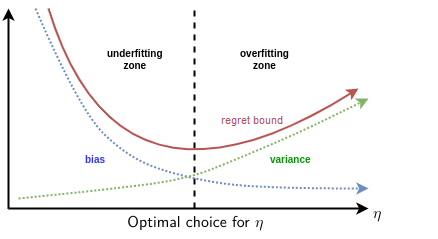
\includegraphics[width=0.9\linewidth]{figure/bias-variance-tradeoff} 
			\end{figure}
			
		\end{minipage}
		%	
		%		
		 \item  {\visible<2-3>{ \textbf{Corollary:}
		%	
		Suppose we use the FTRL algorithm with the squared L2-norm regularization on an online linear optimization problem with $\Aspace \subset \mathbb{R}^d$ such that 
%		
		\begin{itemize}\small
%			
			\item $\sup_{\tilde a \in \Aspace}\norm{\tilde a} \leq B$ for some finite constant $B>0,$ 
%			
			\item $\sup_{z \in \Zspace}\norm{z} \leq V$ for some finite constant $V>0.$
%			
		\end{itemize}
		%	
		Then, by choosing the step size $\eta$ for FTRL as $\eta = \frac{B}{V\sqrt{2\, T}}$ it holds that
		%	
			$$	R_T^{FTRL} \leq   BV\sqrt{2\, T}.		$$
			%	
		 }}
		%		
		\item  {\visible<3>{ Note that the (optimal) parameter $\eta$ depends on the time horizon $T,$ which is oftentimes not known in advance.
		%	
		However, there are some tricks (i.e., the \emph{doubling trick}), which can help in such cases. }}
		%	provides an algorithm which has the same order of the regret, but does not need the knowledge of the time horizon in advance.
		%		
	\end{itemize}
\end{frame}

\begin{frame} 
	\frametitle{FTRL for OLO: Theoretical guarantees}
	\small
	\begin{itemize}	 
		\small
		\item \textbf{Proof:}
		
		\begin{itemize} \small
			%	
			\item By the latter {\color{green} proposition} and the {\color{olive} assumptions }
			%	
			\begin{align*}
				%	
				R_T^{FTRL}(\tilde a)  
				%				 
				 \quad &{\color{green}\leq} \quad  \frac{1}{2\eta}  \norm{\tilde a}^2 \ &&+  \eta  \sum\limits_{t=1}^T \norm{z_t}^2 \\
				%				 
				%				&\leq \frac{1}{2\eta}  \underbrace{\norm{\tilde a}^2}_{\mbox{$\leq B^2$ by assumption}} \ +  \eta  \sum\limits_{t=1}^T \underbrace{\norm{z_t}^2 }_{\mbox{$\leq V^2$ by assumption}} \\
				%		
				 &{\color{olive} \leq} \quad \frac{B^2}{2\eta} \qquad \qquad\qquad\qquad\quad  &&+ \eta \, T \, V^2.
				%		
			\end{align*}
			%	
			 {\visible<2->{	\item The right-hand side of the latter display is independent of $\tilde a,$ so that 
			%	
			\begin{align*}
				%	
				R_T^{FTRL}	\leq   \frac{B^2}{2\eta}  +  \eta \, T \, V^2.
				%		
			\end{align*} }}
			%
			  {\visible<3->{ \item Now, the right-hand side of the latter display is a function of the form $f(\eta) = a/\eta + b \eta$ for some suitable $a,b>0.$ }}
			%	
			 {\visible<3->{ \item   Minimizing $f$ with respect to $\eta$ results in the minimizer $\eta^* = \frac{B}{V\sqrt{2\,T}}.$ }}
			%	
			  {\visible<3->{ \item Plugging this minimizer into the latter display leads to the asserted inequality. \qed }}	
			%	
		\end{itemize}
		%
	\end{itemize}
	%
\end{frame}

\begin{frame}
	\frametitle{Desired results}
	%	
	\small
	\begin{itemize}\small
		%		
		\item With the FTRL algorithm we can cope with 
%		
		\begin{itemize}\small
			%			
			 \item online quadratic optimization (OQO) problems by using no regularity ($\reg \equiv 0$). In this case, we have satisfactory regret guarantees and also a quick update rule for $a_{t+1}^{\FTRL}$ (It is just the empirical average over all data points seen till $t$),
			%			
			 {\visible<2->{  \item online linear optimization (OLO) problems by using a suitable regularization function.
			%			
			In this case, we have quick update formulas and satisfactory regret guarantees as well. }}
			%
		\end{itemize}
		%		
		   \item [$\Rightarrow$]  {\visible<3->{ But what about other online learning problems or rather other loss functions? }}
		%
		 {\visible<3>{   \item  What we wish to have is an approach such that we can achieve for a large class of loss functions $\l$ the advantages of FTRL for OLO and OCO problems:
		
		\begin{itemize}\small
			 \item  [(a)] reasonable regret upper bounds;
			  \item  [(b)] a quick update formula.
		\end{itemize} }}
		%		
%		 \item For this purpose, we will dig into the theory of \emph{convex functions} in order to transfer the advantages of FTRL to a larger class of online learning problems.
		%
	\end{itemize}
	%	
\end{frame}


%
%\begin{frame} 
%	{Summary}
%	%	
%	\footnotesize
%	\begin{itemize}[leftmargin=3.5mm]
%		%		
%		\item We have introduced the (basic) online learning problem in a formal way and defined it based on mainly three components:
%		%
%		\begin{itemize}[leftmargin=3.5mm]
%			%	
%			 \item the environment and the corresponding environmental data space $\Zspace;$
%			%	
%			 \item the learner and its available action space $\Aspace;$
%			%	
%			 \item a loss function to evaluate the actions of the learner for the realized environmental data.
%			%	
%		\end{itemize}
%		%
%		 \item In order to measure the quality or the achievement of a learner over time, we defined the cumulative regret, which is the excess of total loss of the learner over the best action in hindsight.
%		%
%		 \item The goal of the learner is then determined by achieving a reasonable low cumulative regret, for which a suitable adaption on the environment is needed.
%		%
%		 \item We brought the online learning framework to life by considering two examples and showed how these can be cast into the latter:
%		%
%		\begin{itemize}[leftmargin=3.5mm]
%			%	
%			 \item \emph{Weather forecast ---} Predicting the temperature for some locations based on previously observed weather data.
%			%			 \item \emph{Sequential investment ---} Allocating capital on the financial market such that the capital increases over time as much as possible.
%			%
%			 \item \emph{Path planning ---} Finding the optimal path between two nodes in a network/graph structure. Examples are route planning applications or network management systems.
%			%	
%			%			 \item \emph{Online classification problems ---} Observing different object in each time step and deciding on the fly which class/category the objects belong to. Instances are: Spam-filter systems, chat-bots or autonomous driving.
%			%	
%			%			 \item \emph{Click-trough rate prediction ---} Optimizing the website contents for specific users to generate as much clicks as possible.
%			%	
%			%			 \item \emph{Weather forecast ---} Predicting the weather by incorporating additional side information in form of expert advice (predictions) into the own prediction mechanism.
%			%	
%			
%		\end{itemize}
%		%
%		%		 \item We have seen that this is not always possible (without further assumptions/restrictions).
%		%
%	\end{itemize}
%	%	
%\end{frame}


%\begin{frame}
%\frametitle{Summary}
%%	
%\footnotesize
%\begin{itemize}
%	%		
%	\item We have introduced the straightforward extension of batch-learning scenario algorithms for the online learning scenario: The Follow the leader (FTL) algorithm, which chooses in each time step the action which suffers the smallest cumulative loss for the data observed so far.
%	%		
%	 \item We have seen that the FTL algorithm works well for online quadratic optimization (OQO) problems, which we have identified as an important practical application (weather forecast).
%	%		\\
%	 \item However, FTL has many drawbacks:
%	
%	\begin{itemize}
%		%			
%		 \item It might have high computational costs!
%		%			
%		 \item It might not work properly for online linear optimization (OLO) problems such as path planning.
%		%		
%	\end{itemize}
%	%	
%	 \item As a remedy, we defined the Follow the regularized leader (FTRL) algorithm, which involves a regularization component in order to stabilize the action determination mechanism of FTL.
%	%		
%	 \item  Choosing the later component appropriately  leads to a better behavior for online linear optimization (OLO) problems and provides convenient update formulas.
%	%		
%\end{itemize}
%%	
%\end{frame}


%
\endlecture
\end{document}
